% Course-compliant submission: 11 pt, single spacing, one-inch margins.
% The restrained title rules/section headings are inspired by NeurIPS;
% the official NeurIPS class is not used because its format differs.
\documentclass[11pt,letterpaper]{article}
\usepackage[T1]{fontenc}
\usepackage[utf8]{inputenc}
\usepackage{lmodern}
\usepackage[margin=1in]{geometry}
\usepackage{microtype,amsmath,booktabs,graphicx,float}
\usepackage[font=normalsize,labelfont=bf,skip=4pt]{caption}
\usepackage{titlesec}
\usepackage[numbers]{natbib}
\usepackage[hidelinks]{hyperref}
\hypersetup{pdftitle={Progress Report: Privacy-Fairness Tradeoffs},pdfauthor={Xiyin Xu and Shannon Saad}}
\linespread{1}
\setlength{\parindent}{0pt}
\setlength{\parskip}{4pt}
\titleformat{\section}{\normalfont\normalsize\bfseries}{\thesection}{0.6em}{}
\titlespacing*{\section}{0pt}{8pt}{3pt}
\setlength{\intextsep}{7pt}
\graphicspath{{figures/}}
\newcommand{\eps}{\varepsilon}
\begin{document}
\begin{center}
\hrule height 1pt\vspace{5pt}
{\large\bfseries Privacy--Fairness Tradeoffs in DP-SGD\\Employment Prediction}\par
\vspace{4pt}
Xiyin Xu \qquad Shannon Saad\\
ECE 285 Progress Report \quad | \quad November 18, 2026
\vspace{5pt}\hrule height 0.5pt
\end{center}
\vspace{-3pt}

\section{Proposal feedback, updates, and changes}
Our proposal received positive feedback, with encouragement to include additional Folktables datasets. Only ACSEmployment experiments are complete; repeated ACSIncome comparisons are planned next. The original questions remain: does DP-SGD disproportionately reduce group accuracy, can pre-/post-processing mitigate disparities, and how do tradeoffs vary with privacy budget? This extends Bagdasaryan et al.~\cite{bagdasaryan2019} to tabular data and additional fairness criteria.

Implementation refinements are a fixed California/year cohort, removal of the mostly inapplicable ESP feature, and separate reference/development/calibration partitions in addition to training/test data. The objectives and planned Learning Fair Representations (LFR) and equalized-odds (EO) interventions are unchanged.

\section{Experiments completed}
We built a reproducible pipeline for California 2018 ACS 1-Year person data via Folktables~\cite{ding2021}. Filtering to ages 17--89 and positive person weights retains 302,640 of 378,817 records. The target is exactly $Y=1$ for ESR=1 (civilian employed, at work); negatives include temporary absence and military employment. We dropped ESP, missing in 98.58\% of eligible records, without removing people. Fourteen inputs become 77 columns using standardized age and one-hot encoding; sex/race are audit metadata, not direct inputs.

Fixed person-level splits (seed 285) allocate 10\% reference, 50\% training, 10\% development, 10\% calibration, and 20\% test. Preprocessing is fitted only on reference data. We trained an ordinary SGD MLP ($77\!\rightarrow\!64\!\rightarrow\!32\!\rightarrow\!1$, ReLU) and three DP-SGD pilots. All use binary cross-entropy, learning rate 0.05, nominal batch size 512, 20 epochs, and threshold 0.5. DP uses Opacus, Poisson sampling, clipping norm 1, 5,920 updates, and R\'enyi-DP accounting with $\delta=6.61\times10^{-7}$. Smaller $\eps$ means stronger privacy at this fixed $\delta$.

\begin{table}[H]
\centering
\begin{tabular}{lrrrr}\toprule
Method & Achieved $\eps$ & Accuracy & Balanced acc. & Loss (pp)\\\midrule
SGD & --- & 77.08\% & 75.73\% & 0.00\\
DP-SGD & 0.999 & 75.82\% & 73.67\% & 1.26\\
DP-SGD & 3.999 & 75.81\% & 73.69\% & 1.27\\
DP-SGD & 8.000 & 75.78\% & 73.63\% & 1.30\\\bottomrule
\end{tabular}
\caption{Single-run development results; loss is relative to SGD.}\label{tab:results}
\end{table}
The baseline exceeds majority prediction (57.01\% accuracy). Each privacy budget applies to one model-training run, conditional on fixed public reference/development/calibration data. The ordinary baseline is not private. Final test records remain untouched; fairness interventions have not yet been fitted.

\newpage
\section{Important observations and current limitations}
DP training costs about 1.3 accuracy points (Table~\ref{tab:results}). Females lose 1.6--1.7 points versus 0.9 for males (Figure~\ref{fig:groups}). These suggest unequal costs, but the private runs differ by only 0.04 points overall; budget effects require repeated runs.

\begin{figure}[H]
\centering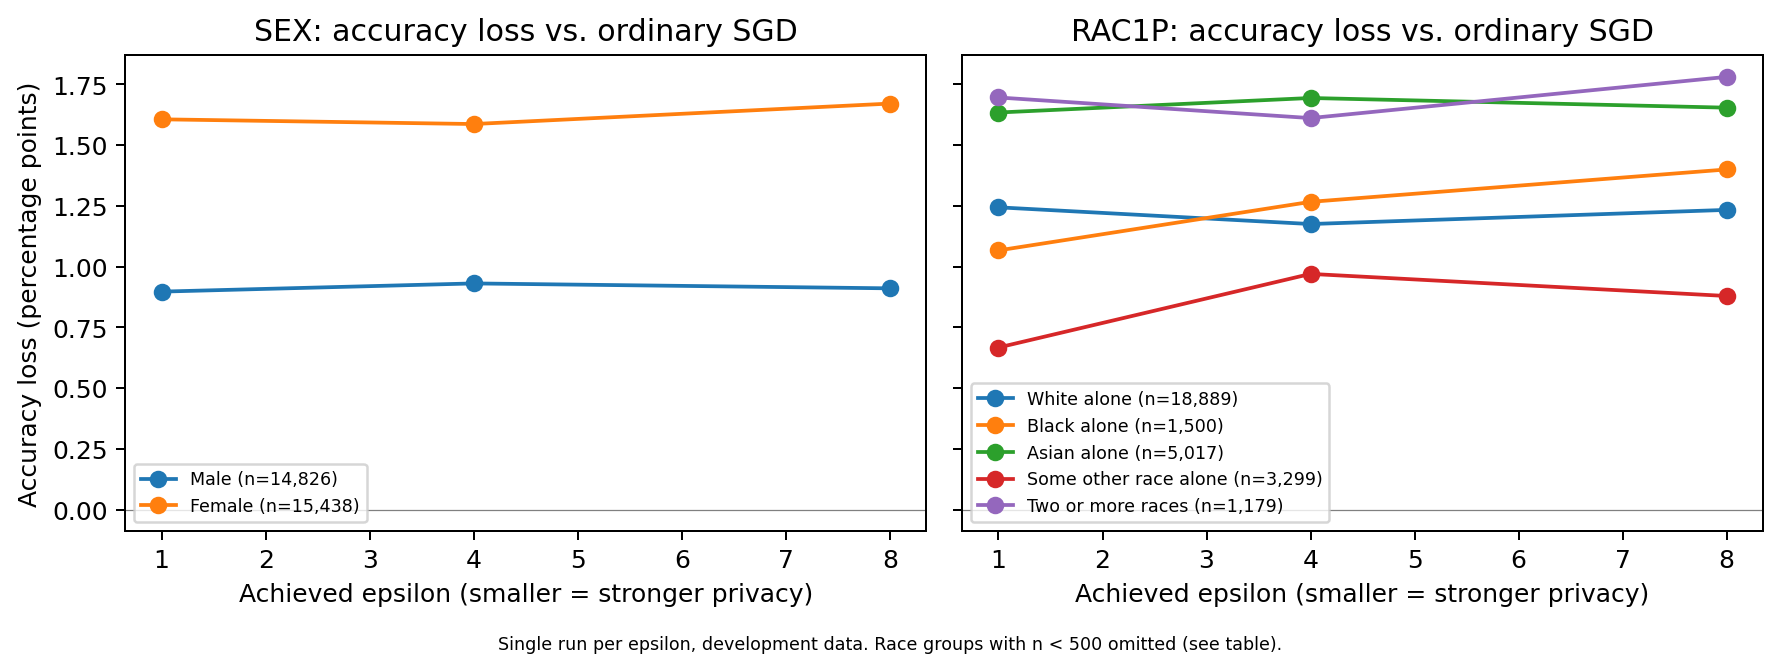
\includegraphics[width=\linewidth]{group_loss_vs_epsilon.png}
\caption{Group accuracy loss versus SGD. Original Census race categories are retained; groups with fewer than 500 development records are omitted only from this display.}\label{fig:groups}
\end{figure}

We measure accuracy parity (equal correctness), independence (equal positive-prediction rates), separation (equal TPR/FPR within actual classes), and binary sufficiency (equal PPV/NPV within predicted classes). Each rate gap is maximum minus minimum across groups; separation/sufficiency take the larger component gap. At $\eps\approx1$, the sex accuracy gap rises from 6.67 to 7.38 points, but separation falls from 12.01 to 11.38 and sufficiency from 12.58 to 12.12: the criteria move in opposite directions.

Full-race separation/sufficiency are undefined because a rare group lacks positive labels, not because disparity is zero. Limitations include single runs, small groups, unweighted metrics, and one task/state/year. Sampling, clipping, and noise differ between ordinary/private training; diagnostics are needed to separate effects. Disparities do not establish causal discrimination.

\section{Remaining steps and timeline}
\textbf{Nov.\ 19--24:} repeat SGD and DP pilots ($\eps=1,4,8$), at least three training seeds per setting, with fixed splits/settings. Report mean accuracy/fairness, standard deviations, and error bars. Fit EO~\cite{hardt2016} (Nov.\ 19--21) and LFR~\cite{zemel2013} (Nov.\ 22--24), with ordinary/private controls.

\textbf{Nov.\ 25--30:} freeze settings; repeat interventions at $\eps\in\{0.5,1,2,4,8\}$ (fallback $\{1,4,8\}$), at least three seeds each; add repeated ACSIncome baseline/DP comparisons. \textbf{Dec.\ 1--3:} final test evaluation and uncertainty estimates. \textbf{Dec.\ 4--7:} write and submit the final report.

\renewcommand{\refname}{References}
\begin{thebibliography}{4}
\setlength{\itemsep}{0pt}\setlength{\parskip}{0pt}
\bibitem{bagdasaryan2019} E.\ Bagdasaryan et al.\ Differential Privacy Has Disparate Impact on Model Accuracy. \textit{NeurIPS}, 2019.
\bibitem{ding2021} F.\ Ding et al.\ Retiring Adult: New Datasets for Fair Machine Learning. \textit{NeurIPS}, 2021.
\bibitem{hardt2016} M.\ Hardt et al.\ Equality of Opportunity in Supervised Learning. \textit{NeurIPS}, 2016.
\bibitem{zemel2013} R.\ Zemel et al.\ Learning Fair Representations. \textit{ICML}, 2013.
\end{thebibliography}
\end{document}
